\documentclass[journal,12pt,twocolumn]{IEEEtran}

\usepackage{setspace}
\usepackage{gensymb}
\singlespacing
\usepackage[cmex10]{amsmath}

\usepackage{amsthm}

\usepackage{mathrsfs}
\usepackage{txfonts}
\usepackage{stfloats}
\usepackage{bm}
\usepackage{cite}
\usepackage{cases}
\usepackage{subfig}

\usepackage{longtable}
\usepackage{multirow}

\usepackage{enumitem}
\usepackage{mathtools}
\usepackage{steinmetz}
\usepackage{tikz}
\usepackage{circuitikz}
\usepackage{verbatim}
\usepackage{tfrupee}
\usepackage[breaklinks=true]{hyperref}
\usepackage{graphicx}
\usepackage{tkz-euclide}

\usetikzlibrary{calc,math}
\usepackage{listings}
    \usepackage{color}                                            %%
    \usepackage{array}                                            %%
    \usepackage{longtable}                                        %%
    \usepackage{calc}                                             %%
    \usepackage{multirow}                                         %%
    \usepackage{hhline}                                           %%
    \usepackage{ifthen}                                           %%
    \usepackage{lscape}     
\usepackage{multicol}
\usepackage{chngcntr}

\DeclareMathOperator*{\Res}{Res}

\renewcommand\thesection{\arabic{section}}
\renewcommand\thesubsection{\thesection.\arabic{subsection}}
\renewcommand\thesubsubsection{\thesubsection.\arabic{subsubsection}}

\renewcommand\thesectiondis{\arabic{section}}
\renewcommand\thesubsectiondis{\thesectiondis.\arabic{subsection}}
\renewcommand\thesubsubsectiondis{\thesubsectiondis.\arabic{subsubsection}}


\hyphenation{op-tical net-works semi-conduc-tor}
\def\inputGnumericTable{}                                 %%

\lstset{
%language=C,
frame=single, 
breaklines=true,
columns=fullflexible
}
\begin{document}


\newtheorem{theorem}{Theorem}[section]
\newtheorem{problem}{Problem}
\newtheorem{proposition}{Proposition}[section]
\newtheorem{lemma}{Lemma}[section]
\newtheorem{corollary}[theorem]{Corollary}
\newtheorem{example}{Example}[section]
\newtheorem{definition}[problem]{Definition}

\newcommand{\BEQA}{\begin{eqnarray}}
\newcommand{\EEQA}{\end{eqnarray}}
\newcommand{\define}{\stackrel{\triangle}{=}}
\bibliographystyle{IEEEtran}
\raggedbottom
\setlength{\parindent}{0pt}
\providecommand{\mbf}{\mathbf}
\providecommand{\pr}[1]{\ensuremath{\Pr\left(#1\right)}}
\providecommand{\qfunc}[1]{\ensuremath{Q\left(#1\right)}}
\providecommand{\sbrak}[1]{\ensuremath{{}\left[#1\right]}}
\providecommand{\lsbrak}[1]{\ensuremath{{}\left[#1\right.}}
\providecommand{\rsbrak}[1]{\ensuremath{{}\left.#1\right]}}
\providecommand{\brak}[1]{\ensuremath{\left(#1\right)}}
\providecommand{\lbrak}[1]{\ensuremath{\left(#1\right.}}
\providecommand{\rbrak}[1]{\ensuremath{\left.#1\right)}}
\providecommand{\cbrak}[1]{\ensuremath{\left\{#1\right\}}}
\providecommand{\lcbrak}[1]{\ensuremath{\left\{#1\right.}}
\providecommand{\rcbrak}[1]{\ensuremath{\left.#1\right\}}}
\theoremstyle{remark}
\newtheorem{rem}{Remark}
\newcommand{\sgn}{\mathop{\mathrm{sgn}}}
\providecommand{\res}[1]{\Res\displaylimits_{#1}} 
%\providecommand{\norm}[1]{\lVert#1\rVert}
\providecommand{\mtx}[1]{\mathbf{#1}}
\providecommand{\fourier}{\overset{\mathcal{F}}{ \rightleftharpoons}}
%\providecommand{\hilbert}{\overset{\mathcal{H}}{ \rightleftharpoons}}
\providecommand{\system}{\overset{\mathcal{H}}{ \longleftrightarrow}}
	%\newcommand{\solution}[2]{\textbf{Solution:}{#1}}
\newcommand{\solution}{\noindent \textbf{Solution: }}
\newcommand{\cosec}{\,\text{cosec}\,}
\providecommand{\dec}[2]{\ensuremath{\overset{#1}{\underset{#2}{\gtrless}}}}
\newcommand{\myvec}[1]{\ensuremath{\begin{pmatrix}#1\end{pmatrix}}}
\newcommand{\mydet}[1]{\ensuremath{\begin{vmatrix}#1\end{vmatrix}}}
\numberwithin{equation}{subsection}
\makeatletter
\@addtoreset{figure}{problem}
\makeatother
\let\StandardTheFigure\thefigure
\let\vec\mathbf
\renewcommand{\thefigure}{\theproblem}
\def\putbox#1#2#3{\makebox[0in][l]{\makebox[#1][l]{}\raisebox{\baselineskip}[0in][0in]{\raisebox{#2}[0in][0in]{#3}}}}
     \def\rightbox#1{\makebox[0in][r]{#1}}
     \def\centbox#1{\makebox[0in]{#1}}
     \def\topbox#1{\raisebox{-\baselineskip}[0in][0in]{#1}}
     \def\midbox#1{\raisebox{-0.5\baselineskip}[0in][0in]{#1}}
\pagenumbering{gobble}
\title{Assignment-2}
\author{Adil Salfi  - CS20BTECH11031}
\maketitle
Download all python codes from
\begin{lstlisting}
https://github.com/AdilSalfi/AI1103/tree/main/Assignment-2/Codes
\end{lstlisting}
and latex-tikz code from
\begin{lstlisting}
https://github.com/AdilSalfi/AI1103/tree/main/Assignment-2
\end{lstlisting}
\section*{\textbf{Problem}}
GATE-EC Question 59 : \\
Let X be a random variable having the distribution function :
\begin{align*}
F(x)=   
\begin{cases}
0 & x<0 \\
\frac{1}{4} & 0\le x<1 \\
\frac{1}{3} & 1\le x<2 \\
\frac{1}{2} & 2\le x<\frac{11}{3} \\
1 & x\ge\frac{11}{3}
\end{cases}
\end{align*}
\section*{\textbf{Solution}}

\begin{definition}[Heaviside step function]
Heaviside step function $u(x)$ is 
\begin{align*}
u(x)=               \tag{1} \label{1}
    \begin{cases}
    0 & x<0 \\
    1 & x\geq 0
    \end{cases}
\end{align*}
Using the Heaviside step function $u(x)$, a function $F(t)$ can be obtained whose output is $f(t)$ for the interval $[a,b)$ and $0$ everywhere else
\begin{align*}
    F(t)=f(t)[u(t-a) - u(t-b)] \tag{2} \label{2}
\end{align*}
\end{definition}

\begin{definition}[Dirac delta function]
Dirac delta function is the derivative of the Heaviside step function $u(x)$
\begin{align*}
    \delta(x) = \frac{du(x)}{dx} \tag{3} \label{3}
\end{align*}
An important property of the Dirac delta function is 
\begin{align*}
    \int_{-\infty}^{\infty}f(x)\delta(x-x_0)dx = f(x_0) \tag{4} \label{4}
\end{align*}
\end{definition}


% \textrightarrow Let us define the Heaviside step function $u(x)$
% \begin{align*}
% u(x)=
% \begin{cases}
% 0 & x<0 \\
% 1 & x\geq 0
% \end{cases}
% \end{align*}
% \textrightarrow The Heaviside step function can be used to obtain a function $F(t)$ whose output is  $f(t)$ for the interval $[a,b)$ and $0$ everywhere else using the the property
% \begin{equation*}
% F(t)=f(t)[u(t-a)-u(t-b)] \tag{1} \label{1}
% \end{equation*}
% \textrightarrow The derivative of the Heaviside step function $u(x)$ is the dirac delta function $\delta(x)$
% \begin{equation*}
% \delta(x)=\frac{du(x)}{dx} \tag{2} \label{2}
% \end{equation*}
% \textrightarrow An important property of the delta function is 
% \begin{equation*}
% \int_{-\infty}^{\infty} f(x)\delta(x-x_0)dx=f(x_0) \tag{3} \label{3}
% \end{equation*}
\textrightarrow To obtain the CDF $F(x)$ in terms of Heaviside step function $u(x)$, we use \eqref{2}
\begin{multline*}
F(x)=\frac{1}{4}[u(x)-u(x-1)]+\frac{1}{3}[u(x-1)-u(x-2)]+\\
\frac{1}{2}[u(x-2)-u(x-\frac{11}{3}]+u(x-\frac{11}{3})
\end{multline*}
\begin{align*}
\implies F(x)=\frac{u(x)}{4}+\frac{u(x-1)}{12}+\frac{u(x-2)}{6}+\frac{u(x-\frac{11}{3})}{2} \tag{5} \label{5}
\end{align*}
\textrightarrow To obtain PDF $f(x)$ we differentiate \eqref{5} and using \eqref{3}, we get
\begin{align*}
f(x)=\frac{\delta(x)}{4}+\frac{\delta(x-1)}{12}+\frac{\delta(x-2)}{6}+\frac{\delta(x-\frac{11}{3})}{2} \tag{6} \label{6}
\end{align*}
\textrightarrow To obtain $E(x)$ we use the formula
\begin{equation*}
E(x)=\int_{-\infty}^{\infty} xf(x)dx \tag{7} \label{7}
\end{equation*}
\textrightarrow Substituting \eqref{6} in \eqref{7}, we get
\begin{multline*}
E(x)=\int_{-\infty}^{\infty} \frac{x}{4}\delta(x)+\int_{-\infty}^{\infty} \frac{x}{12}\delta(x-1)+\int_{-\infty}^{\infty} \frac{x}{6}\delta(x-2)+\\ 
\int_{-\infty}^{\infty} \frac{x}{2}\delta(x-\frac{11}{3}) 
\end{multline*}
\textrightarrow Using \eqref{4}, we get
\begin{align*}
E(x)&=\frac{0}{4}+\frac{1}{12}+\frac{2}{6}+\frac{\frac{11}{3}}{2} \\
\therefore E(x)&=2.25 
\end{align*}
\newpage
\begin{figure}[h!]
    \centering
    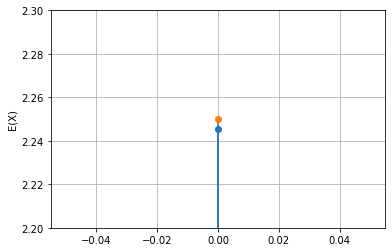
\includegraphics[width=\columnwidth]{plot.png}
    \label{fig:1}
    \figuretag{Fig. 1:Plot comparing Simulated and Theoretical value of $E(x)$}
\end{figure}
\end{document}
